\ylDisplay{Läätse fookuskaugus} % Ülesande nimi
{Tundmatu autor} % Autor
{lõppvoor} % Voor
{2014} % Aasta
{P 9} % Ülesande nr.
{3} % Raskustase
{
% Teema: Valgusõpetus
\ifStatement
Nõguspeegliga puutub tihedalt kokku kumerlääts. Optilisel peateljel asub valguspunkt $S$. Valguspunktist väljuvad kiired läbivad läätse, peegelduvad peeglilt ja läbides uuesti läätse koonduvad samas punktis $S$. Arvutage läätse fookuskaugus, kui peegli kõverusraadius on $1$ m ja punkt $S$ asub läätsest $20$ cm kaugusel.
\fi
\ifHint
Kuna kiired lähtuvad punktist $S$ ja koonduvad uuesti punktis $S$, on $S$ optilise süsteemi fookuseks. Nõguspeegli ja kumerläätse optilised tugevused liituvad.
\fi
\ifSolution
Kuna kiired lähtuvad punktist $S$ ja koonduvad uuesti punktis $S$, on $S$ optilise süsteemi fookuseks. \\
Seega süsteemi optiline tugevus on $D = \frac{1}{0,2 m} + \frac{1}{0,2 m} =$ $10$ dpt. \\
Kuivõrd süsteemi optiline tugevus võrdub $D = 2D_1 + D_2$ 
ja nõguspeegli optiline tugevus $D_2 =$ $2$ dpt, sest $f = \frac{R}{2}$, siis läätse optiline tugevus on $4$ dpt ja fookuskaugus $f =$ $25$ cm.
\begin{center}
	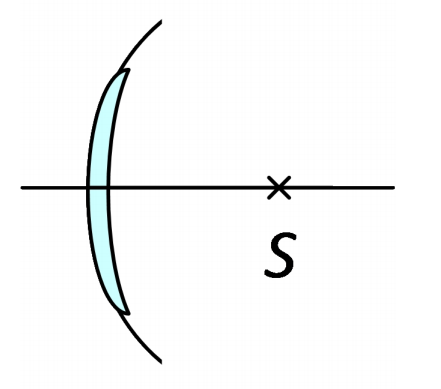
\includegraphics[width=0.5\linewidth]{2014-v3p-09-lah.PNG}
\end{center}
\fi
}